\documentclass[man,floatsintext]{apa6}
\usepackage{lmodern}
\usepackage{amssymb,amsmath}
\usepackage{ifxetex,ifluatex}
\usepackage{fixltx2e} % provides \textsubscript
\ifnum 0\ifxetex 1\fi\ifluatex 1\fi=0 % if pdftex
  \usepackage[T1]{fontenc}
  \usepackage[utf8]{inputenc}
\else % if luatex or xelatex
  \ifxetex
    \usepackage{mathspec}
  \else
    \usepackage{fontspec}
  \fi
  \defaultfontfeatures{Ligatures=TeX,Scale=MatchLowercase}
\fi
% use upquote if available, for straight quotes in verbatim environments
\IfFileExists{upquote.sty}{\usepackage{upquote}}{}
% use microtype if available
\IfFileExists{microtype.sty}{%
\usepackage{microtype}
\UseMicrotypeSet[protrusion]{basicmath} % disable protrusion for tt fonts
}{}
\usepackage{hyperref}
\hypersetup{unicode=true,
            pdftitle={Manuscript Draft},
            pdfauthor={Sally E. Claridge, Daniel M. Charytonowicz, \& Adam A. Margolin},
            pdfkeywords={keywords},
            pdfborder={0 0 0},
            breaklinks=true}
\urlstyle{same}  % don't use monospace font for urls
\usepackage{graphicx,grffile}
\makeatletter
\def\maxwidth{\ifdim\Gin@nat@width>\linewidth\linewidth\else\Gin@nat@width\fi}
\def\maxheight{\ifdim\Gin@nat@height>\textheight\textheight\else\Gin@nat@height\fi}
\makeatother
% Scale images if necessary, so that they will not overflow the page
% margins by default, and it is still possible to overwrite the defaults
% using explicit options in \includegraphics[width, height, ...]{}
\setkeys{Gin}{width=\maxwidth,height=\maxheight,keepaspectratio}
\IfFileExists{parskip.sty}{%
\usepackage{parskip}
}{% else
\setlength{\parindent}{0pt}
\setlength{\parskip}{6pt plus 2pt minus 1pt}
}
\setlength{\emergencystretch}{3em}  % prevent overfull lines
\providecommand{\tightlist}{%
  \setlength{\itemsep}{0pt}\setlength{\parskip}{0pt}}
\setcounter{secnumdepth}{0}
% Redefines (sub)paragraphs to behave more like sections
\ifx\paragraph\undefined\else
\let\oldparagraph\paragraph
\renewcommand{\paragraph}[1]{\oldparagraph{#1}\mbox{}}
\fi
\ifx\subparagraph\undefined\else
\let\oldsubparagraph\subparagraph
\renewcommand{\subparagraph}[1]{\oldsubparagraph{#1}\mbox{}}
\fi

%%% Use protect on footnotes to avoid problems with footnotes in titles
\let\rmarkdownfootnote\footnote%
\def\footnote{\protect\rmarkdownfootnote}


  \title{Manuscript Draft}
    \author{Sally E. Claridge\textsuperscript{1}, Daniel M.
Charytonowicz\textsuperscript{1}, \& Adam A.
Margolin\textsuperscript{1, 2}}
    \date{}
  
\shorttitle{Subtitle}
\affiliation{
\vspace{0.5cm}
\textsuperscript{1} Department of Genetics and Genomic Sciences, Icahn Institute for Data Science and Genomic Technology, Icahn School of Medicine at Mount Sinai, New York, NY\\\textsuperscript{2} Cancer Target Discovery and Development Network (Oregon Health and Science University, Portland, OR), National Cancer Institute, National Institutes of Health}
\keywords{keywords\newline\indent Word count: X}
\usepackage{csquotes}
\usepackage{upgreek}
\captionsetup{font=singlespacing,justification=justified}

\usepackage{longtable}
\usepackage{lscape}
\usepackage{multirow}
\usepackage{tabularx}
\usepackage[flushleft]{threeparttable}
\usepackage{threeparttablex}

\newenvironment{lltable}{\begin{landscape}\begin{center}\begin{ThreePartTable}}{\end{ThreePartTable}\end{center}\end{landscape}}

\makeatletter
\newcommand\LastLTentrywidth{1em}
\newlength\longtablewidth
\setlength{\longtablewidth}{1in}
\newcommand{\getlongtablewidth}{\begingroup \ifcsname LT@\roman{LT@tables}\endcsname \global\longtablewidth=0pt \renewcommand{\LT@entry}[2]{\global\advance\longtablewidth by ##2\relax\gdef\LastLTentrywidth{##2}}\@nameuse{LT@\roman{LT@tables}} \fi \endgroup}


\DeclareDelayedFloatFlavor{ThreePartTable}{table}
\DeclareDelayedFloatFlavor{lltable}{table}
\DeclareDelayedFloatFlavor*{longtable}{table}
\makeatletter
\renewcommand{\efloat@iwrite}[1]{\immediate\expandafter\protected@write\csname efloat@post#1\endcsname{}}
\makeatother
\usepackage{lineno}

\linenumbers

\authornote{Add complete departmental affiliations for each
author here. Each new line herein must be indented, like this line.

Enter author note here.

Correspondence concerning this article should be addressed to Adam A.
Margolin, Icahn School of Medicine at Mount Sinai, Deparment of Genetics
and Genomic Sciences, One Gustave L. Levy Place, Box 1498, New York, NY
10029. E-mail:
\href{mailto:adam.margolin@mssm.edu}{\nolinkurl{adam.margolin@mssm.edu}}}

\abstract{
Multiple high-throughput functional screens in cancer cell lines have
generated large amounts of information on drug efficacy in a variety of
genomic contexts and cancer lineages. Inconsistencies between datasets
have led us to investigate whether these large-scale screens reproduce
established clinical drug-gene associations and if genomic features
particular to specific genes improve said reproducibility. We evaluated
three large-scale, small-molecule drug screens and one CRISPR/Cas9 gene
essentiality screen, all within the context of clinical interpretations
derived from a new cancer variant annotation resource published by the
Variant Interpretation for Cancer Consortium (VICC). We identified low
levels of concordance between the three drug screen datasets and
clinical drug-gene associations using mutation status, gene expression,
and copy number as genomic indicators. Less than half of the clinical
drug-gene cancer associations from the VICC resource were identified in
these three drug screen datasets, suggesting a barrier to translating
findings from these large-scale screens into the clinic.


}

\begin{document}
\maketitle

\section{Introduction}\label{introduction}

Cancer cell lines are a long-standing model for systematic testing of
candidate therapeutics, beginning with the National Cancer Institute 60
(NCI60) assay from the late 1980s (M. C. Alley et al., 1988; R. H.
Shoemaker, 2006; Stinson et al., 1992), which has been used to screen
over 100,000 compounds as of 2010 (Holbeck, Collins, \& Doroshow, 2010).
Since then, numerous small-molecule and gene essentiality screens of
various scales and study aims have been conducted in cell lines, from
grouping drugs by therapeutic target similarity (Greshock et al., 2010)
to screening only near-haploid cell lines to generate genome-level
insights into gene essentiality (T. Wang et al., 2015) to broadly
identifying cancer dependencies with large-scale screens in multiple
cancer types (McDonald et al., 2017; J. M. McFarland et al., 2018;
Meyers et al., 2017; Patel et al., 2017) or select lineages (Heiser et
al., 2009; Marcotte et al., 2012; Patel et al., 2017). Despite their
widespread use, cancer cell lines are known to have issues with
inconsistent naming conventions and contamination (M. Yu et al., 2015),
and some cell lines have been shown to vary widely at the genetic level
and in response to drug treatment across strains (Ben-David et al.,
2018). Additionally, comparisons between cancer cell lines and tumors
indicate that cell lines have higher numbers of genomic aberrations
(Domcke, Sinha, Levine, Sander, \& Schultz, 2013; Mouradov et al., 2014;
Neve et al., 2006) and tend to be hypermethylated (Paz et al., 2003;
Varley et al., 2013), which could prove an impediment to translating
cell line discoveries into the clinic.

There have also been debates over consistency between drug screen
datasets, namely the Broad Institute's and Novartis Institutes for
Biomedical Research's Cancer Cell Line Encyclopedia (CCLE) (J. Barretina
et al., 2012; T. C. C. L. E. Consortium \& Consortium, 2015) and the
Genomics of Drug Sensitivity in Cancer (GDSC) from the Cancer Genome
Project at the Wellcome Sanger Institute and the Center for Molecular
Therapeutics at Massachusetts General Hospital Cancer Center (Garnett et
al., 2012; Yang et al., 2012). The GDSC has also been referred to as the
Cancer Genome Project (CGP) and the Sanger dataset. Studies have shown
that drug-gene interactions matched between CCLE and GDSC exhibited poor
correlation and inconsistencies (Haibe-Kains et al., 2013; Jang, Neto,
Guinney, Friend, \& Margolin, 2014), prompting other groups to join the
debate on how best correct for experimental and methodological variation
between the original drug screens and subsequent computational analysis
(T. C. C. L. E. Consortium \& Consortium, 2015; Geeleher, Cox, \& Huang,
2016; Geeleher, Gamazon, Seoighe, Cox, \& Huang, 2016; Hatzis et al.,
2014; Haverty et al., 2016; Safikhani et al., 2016, 2017).

The prevalence and importance of cancer cell lines in large-scale
therapeutic research and the apparent inconsistencies between the GDSC
and CCLE encouraged us to compare the results from these functional
screens to clinical drug-gene associations. An outstanding question
concerning studies based on cancer cell lines is whether these the cell
line systems can accurately model tumor dynamics or recapitulate
clinical cancer vulnerabilities, and many large-scale grants and
clinical trials are fundamentally anchored by results from screens
conducted in cancer cell lines. Thus, our goal was to evaluate how well
these functional screens recapitulate known drug, gene, and tumor type
associations that are currently used in clinical decision-making.

We derived our clinical associations from a new project conducted by the
Variant Interpretation for Cancer Consortium (VICC;
\url{https://cancervariants.org/}), a Driver Project for the Global
Alliance for Genomics and Health (GA4GH) (The Global Alliance for
Genomics and Health, 2016). The VICC has curated annotations of known
cancer variants at varying levels of evidence from multiple resources
(A. H. Wagner et al., 2018): the Precision Medicine Knowledgebase (L.
Huang et al., 2016), MolecularMatch
(\url{https://www.molecularmatch.com/index.html}), OncoKB (Chakravarty
et al., 2017), Jackson Labs Clinical Knowledgebase (S. E. Patterson et
al., 2016), Clinical Interpretations of Variance in Cancers (CIViC)
(Griffith et al., 2017), and the Cancer Genome Interpreter (CGI)
(Tamborero et al., 2018). These harmonized variants are hosted on an
ElasticSearch (Kibana v6.0) platform called Genotype to Phenotype (G2P,
\url{https://search.cancervariants.org/\#*}) that allows users to query
and filter aggregated evidence from the various databases listed above
as well as the GA4GH beacon service
(\url{http://beacon-network.org/\#/}), which yields access to genetic
mutation data from over 200 datasets as of 2016 (The Global Alliance for
Genomics and Health, 2016). For drug screen datasets, we focus on three
well-known, large-scale drug projects: the CCLE and GDSC, which were
mentioned above, and the Center for the Science of Therapeutics at the
Broad Institute's Cancer Therapeutics Response Portal (CTRP) dataset
(Basu et al., 2013; M. G. Rees et al., 2016; B. Seashore-Ludlow et al.,
2015). We also analyzed the results from a large-scale CRISPR/Cas9
screen conducted by the Broad Institute's Cancer Dependency Map project
(DepMap) using the Avana knockout library (Doench et al., 2016; Meyers
et al., 2017), which will address whether gene essentiality screens via
CRISPR yield results comparable to functional drug screens.

\section{Results}\label{results}

\subsection{Do small-molecule screens in cancer cell lines recapitulate
clinical drug-gene
associations?}\label{do-small-molecule-screens-in-cancer-cell-lines-recapitulate-clinical-drug-gene-associations}

\begin{table}[tbp]
\begin{center}
\begin{threeparttable}
\caption{\label{tab:table-g2p-nonCID}Level-A G2P interpretations excluded from analyses}
\small{
\begin{tabular}{cccc}
\toprule
Compound & \multicolumn{1}{c}{CID} & \multicolumn{1}{c}{N\_G2P} & \multicolumn{1}{c}{\%}\\
\midrule
EGFR & SID160769799 & 1 & 0.25\\
pertuzumab & CHEMBL2007641 & 1 & 0.25\\
ipilimumab & CHEMBL1789844 & 2 & 0.50\\
cisplatin & CHEMBL2068237 & 3 & 0.75\\
pembrolizumab & CHEMBL3137343 & 3 & 0.75\\
nivolumab & CHEMBL2108738 & 4 & 1.00\\
trastuzumab & CHEMBL1201585 & 9 & 2.24\\
mAb & CHEMBL2109423 & 16 & 3.98\\
cetuximab & CHEMBL1201577 & 74 & 18.41\\
panitumumab & CHEMBL1201827 & 75 & 18.66\\
NA & NA & 214 & 53.23\\
\bottomrule
\addlinespace
\end{tabular}
}
\begin{tablenotes}[para]
\normalsize{\textit{Note.} N\_G2P (\%) = number of associated G2P interpretations, \% is out of column total; mAb = monoclonal antibody; NA indicates G2P interpretation does not have an associated compound.}
\end{tablenotes}
\end{threeparttable}
\end{center}
\end{table}

G2P designed a set of standards for stratifying their database's cancer
variant interpretations, ranging from preclinical data at the
low-evidence end (level D) to clinically actionable interpretations at
the high-evidence end (level A). To test only these clinically
actionable associations, we filtered the G2P dataset for only level-A
G2P interpretations, of which there were 1,296 (see Methods). All
compounds screened within the GDSC, CTRP, and CCLE datasets are
considered \enquote{small molecules} and are respectively linked to
Compound (CID) numbers used for indexing in the PubChem database
(\url{https://pubchem.ncbi.nlm.nih.gov/}). As a result, non-small
molecules, which include proteins and biologics (i.e.~monoclonal
antibodies), that had level-A G2P evidence could not be included in our
comparisons. Thus, G2P interpretations for which the compound did not
have a matching CID code were excluded from further analysis as were
interpretations that did not have an associated compound, resulting in
removal of 402 interpretations (Table~\ref{tab:table-g2p-nonCID}). It
should be noted that cisplatin, a small molecule, was excluded due to
its being indexed with a ChEMBLdb identifier
(\url{https://www.ebi.ac.uk/chembl/}), which we did not manually
re-index to a CID to avoid accidental mischaracterization.

After filtering, 894 level-A G2P interpretations were carried forward in
subsequent analyses, constituting 57 unique drugs and 34 unique genes in
88 distinct level-A combinations (\emph{Figure 1A}). The number of
level-A interpretations per drug ranged from 1 to 176 (\(M =\) 15.68,
\(SD =\) 34.63), 1 to 264 (\(M =\) 26.24, \(SD =\) 61.58) per gene, and
for each level-A drug-gene combination, the range was 1 to 103 (\(M =\)
10.14, \(SD =\) 19.80). These unique drugs, genes, and combinations are
hereafter referred to as G2P drugs, G2P genes, and G2P associations.
Filtering our screening datasets by these clinical criteria yields
panels of potentially clinically relevant omic features. Of the 57
unique G2P drugs, 37 of them were screened in at least one of the drug
screen datasets, 17 drugs were screened in at least two of the three
datasets, and only 3 were screened in all three datasets. The remaining
20 un-screened G2P drugs suggests an incompleteness of these drug
screens, though these projects frequently release new screening data
that may include these drugs in future releases.

Using cell-line-specific point mutation annotations from the CCLE, we
compared z-score-transformed area under the dose-response curve (AUC)
distributions between mutant and wildtype cell lines for all G2P
associations tested in the CCLE, CTRP, and GDSC drug screens. Of the 88
G2P associations, data was available for 9 associations in CCLE, 48 in
CTRP, and 44 in GDSC. Controlling for a false discovery rate (FDR)
\textless{} 5\%, CCLE yielded no significant correlations (Wilcoxon
rank-sum tests, \(p_k = 2.1^{-4}\)), though the most significant G2P
association was selumetinib-\emph{KRAS} (\(p_{adj} = 1.9^{-3}\)). In
CTRP, AUC from 3 drug-gene associations correlated with the gene's
mutation status (\(p_k = 4.5^{-3}\)): selumetinib-\emph{KRAS}
(\(p_{adj} = 4.4^{-8}\)), vemurafenib-\emph{BRAF}
(\(p_{adj} = 4.4^{-8}\)), and dabrafenib-\emph{BRAF}
(\(p_{adj} = 7.7^{-5}\)). Dabrafenib-\emph{BRAF}
(\(p_{adj} = 8.6^{-11}\)) and trametinib-\emph{BRAF}
(\(p_{adj} = 4.2^{-6}\)) were significant in GDSC (\(p_k = 2.3^{-3}\)).

\begin{quote}
\textbf{(???) Describe why we compare all pairwise combos rather than
filtering for just the drug-gene combos in G2P?}
\end{quote}

To test for potentially novel drug-gene associations, we conducted
similar Wilcoxon rank-sum tests for all pairwise combinations of G2P
genes and drugs tested in the three drug screens (\emph{Figures 1B and
2A}). At an unadjusted \(\alpha = 0.05\), the tests revealed that in
CCLE, AUC significantly correlated with mutation status for 18 out of
170 (10.59\%) tested drug-gene combinations were significantly
different, 135 out of 918 (14.71\%) were significantly different for
CTRP, and 89 out of 850 (10.47\%) for GDSC.

Controlling for a FDR \textless{} 5\%, selumetinib-\emph{BRAF}
(\(p_{adj} = 1.4^{-10}\)) was the only significant drug-gene combination
tested in CCLE (\(p_k = 7.9^{-4}\)). CTRP (\(p_k = 6.5^{-4}\)) yielded 5
significant combinations, one of which was selumetinib-\emph{BRAF}.
There were 3 significant G2P associations in the GDSC dataset
(\(p_k = 9.5^{-5}\)). Of all the significant correlations between
mutation status and AUC across datasets, the only genes represented were
\emph{KRAS} and \emph{BRAF} (Figure~\ref{fig:drug-venn}). Of the 7
significant drug-gene associations across datasets, 4 were G2P
associations. The remaining 3 associations were selumetinib-\emph{BRAF},
trametinib-\emph{KRAS}, and pazopanib-\emph{BRAF}.

\begin{quote}
\textbf{(???) Trametinib and selumetinib are both \emph{MEK} inhibitors,
and pazopanib is a \emph{VEGFR} inhibitor. VEGF signaling can influence
the MAPK/ERK signaling pathway, which promotes cell proliferation and
survival. This pathway includes \emph{RAS}, \emph{BRAF}, and \emph{MEK}
proteins. These results underscore the importance of the MAPK/ERK
signaling pathway in cancer.}
\end{quote}

However, taking these results as a whole, we observe little concordance
between G2P associations and the correlation of mutation status and AUC
for said G2P association, suggesting that mutation status alone is not a
robust predictor of clinically actionable genetic targets. This led us
to examine the correlations between AUC and gene expression and AUC and
copy number, two other genomic features that are known to associate with
cancer and drug response. We computed Spearman correlation coefficients
(\(r_s\)) between AUC of each drug-gene association and gene expression
(RPKM) and copy number (log\(_2\) ratio) of the gene in the
association\ldots{}

\begin{figure}
\centering
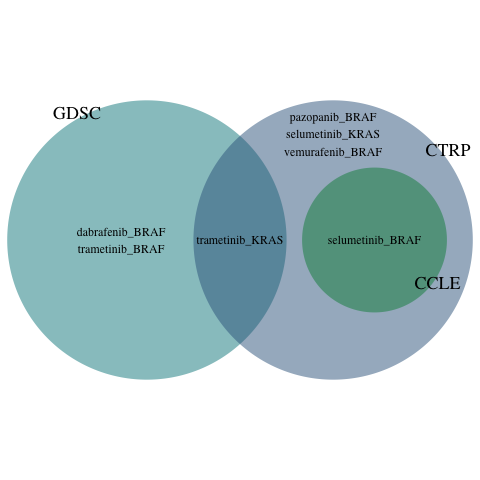
\includegraphics{./plots/manuscript/drugscreen_venn.png}
\caption{}
\end{figure}

\begin{quote}
\textbf{(???) Cut this analysis since we are comparing distributions of
p-values?}
\end{quote}

We compared the distribution of level-A G2P associations (\emph{Figure
1A}) and the associated p-values from the mutation status comparisons
(\emph{Figure 1B}) with a null distribution of p-values derived from all
pairwise combinations of G2P genes and the G2P drugs tested in each
dataset, less any of the 88 distinct combinations with G2P
interpretations, i.e.~the non-gray squares in the right heatmap of
\emph{Figure 1A (Figure 3A}). To formally test concordance between
clinically actionable variants and drug screen results, we conducted an
independent, two-group t-test to compare the distributions of p-values
of drug-gene combinations that either were or were not represented with
level-A evidence in G2P, which indicated that the distributions of
p-values did not significantly differ for CCLE {[}t(9) = 0.25, p =
0.81{]}, CTRP {[}t(51) = 0.85, p = 0.40{]}, nor GDSC {[}t(47) = -0.56, p
= 0.58{]} (Table 2). This further supports that mutation status is not a
robust genomic feature for predicting therapeutic responses.

Similar tests were conducted for the distributions of Pearson
correlation coefficients (r) between the number of level-A G2P
associations and gene expression (RPKM) and copy number (log2 ratio) of
the gene in the association (\emph{Figures 3B-C}). Example r derivations
are shown in \emph{Figures 2B-C}. Absolute values of r were used to
simplify extreme values in both directions for testing. The difference
in the CCLE \textbar{}r\textbar{} distributions for both gene expression
{[}t(8) = 1.43, p = 0.19{]} and copy number {[}t(8) = 2.48, p = 0.23{]}
were non-significant, which is likely explained by the small sample size
since only five G2P drugs were screened in the CCLE dataset. For both
the CTRP and GDSC screens, \textbar{}r\textbar{} values for gene
expression correlations were significantly greater for the level-A G2P
associations than the null distribution {[}tCTRP(49) = 3.79, pCTRP
\textless{} 0.001; tGDSC(44) = 2.97, pGDSC = 0.005{]}. The
\textbar{}r\textbar{} distributions using copy number were also
significantly different for CTRP {[}t(49) = 2.48, p = 0.017{]} but not
for GDSC {[}t(44) = 1.95, p = 0.058{]}.

In all three datasets for both level-A G2P associations and null
distribution associations, there are more significant
\textbar{}r\textbar{} values when using gene expression as the genomic
feature than when using copy number (Table 2), which corresponds with
previous work showing that gene expression is an informative molecular
feature when assessing drug sensitivity (Jang et al., 2014; Sirota et
al., 2011). Additionally, in all cases, there are more significant r
values when using copy number than there are significant p-values from
the mutation status comparisons. Though observational, these results
suggest an order of predictive robustness for these three genomic
features when used in isolation: Gene expression \textgreater{} copy
number \textgreater{} mutation status. Additionally, across all three
genomic features, CTRP consistently identified a higher percentage of
its possible level-A G2P associations than GDSC, and similarly, GDSC
identified a higher percentage than CCLE. In the CCLE-GDSC debate,
inconsistency between the datasets was attributed to the groups using
two very different assays for generating AUC measurements though it was
undecided which was more accurate (Haibe-Kains et al., 2013; Jang et
al., 2014; Weinstein \& Lorenzi, 2013). Our results provide very
preliminary evidence that GDSC is more accurate than CCLE in regards to
reproducing clinical associations. However, CTRP may be even more
accurate than both GDSC and CCLE.

\subsection{Do these pancancer drug-gene associations penetrate to the
lineage-specific
level?}\label{do-these-pancancer-drug-gene-associations-penetrate-to-the-lineage-specific-level}

\begin{itemize}
\tightlist
\item
  What do these correlations with mutation status, gene expression, and
  copy number look like when you constrict to a specific lineage?
\item
  When you restrict, do the correlations become more distinct?
\item
  Are the lineage-specific results approximately the same as the
  pancancer results?
\item
  Looking at a histogram of p-values, if the histogram is flat, then
  nothing is significant (note from meeting on 11/16)
\item
  KS test results
\end{itemize}

In the 894 level-A G2P interpretations, there was a wide variation in
the specificity of cancer description, ranging from \enquote{Waldenström
macroglobulinemia} and \enquote{hyper eosinophilic advanced syndrome} on
the more detailed end to \enquote{cancer} on the broad end. Similarly,
the drug screen datasets had a wide range in lineage specificity,
e.g.~CCLE, GTRP, and GDSC all had lineages labeled \enquote{leukemia}
and \enquote{T-cell childhood acute lymphocytic leukemia} and the CRISPR
dataset had cell lines labeled \enquote{Epstein-Barr virus-related
Burkitt lymphoma} and \enquote{lymphoma.} To more easily conduct
comparative analyses in a cancer-specific manner, we developed a more
general lineage grouping method derived from the Human Disease Ontology
identity codes (DOIDs, \url{http://disease-ontology.org/}) (Schriml et
al., 2019) assigned to each cell line, yielding 27 unique lineage
groupings. This custom lineage grouping was included in our harmonized
cancer cell line database (see Methods).

In the level-A G2P interpretations, there were 102 unique
drug-gene-lineage combinations (DGLs), representing seven of our curated
cancer lineages: cancer, lung cancer, breast cancer, leukemia, thyroid
cancer, skin cancer, and ovarian cancer. CCLE had data for 9 DGLs, CTRP
had data for 61, and GDSC had data for 53, yielding a total of 73 unique
DGLs across all three datasets. Only 7 DGLs were screened in all three
datasets.

Prior to correction for an FDR of 5\%, no DGLs were identified in the
CCLE screen when using mutation status as a correlate (\(n =\) 7, 2 DGLs
were not analyzed due to lack of mutation annotations in \emph{UGT1A1}
in \enquote{cancer} lineages), but CTRP (\(n =\) 48) and GDSC (\(n =\)
39) identified 6 and 5, respectively, in skin cancer, lung cancer, and
cancer. After Benjamini-Hochberg FDR correction, none of the datasets
yielded significant DGL interactions.

\begin{quote}
\textbf{(???) KS test results}
\end{quote}

(Figure~\ref{fig:ksplot})

\begin{figure}
\centering
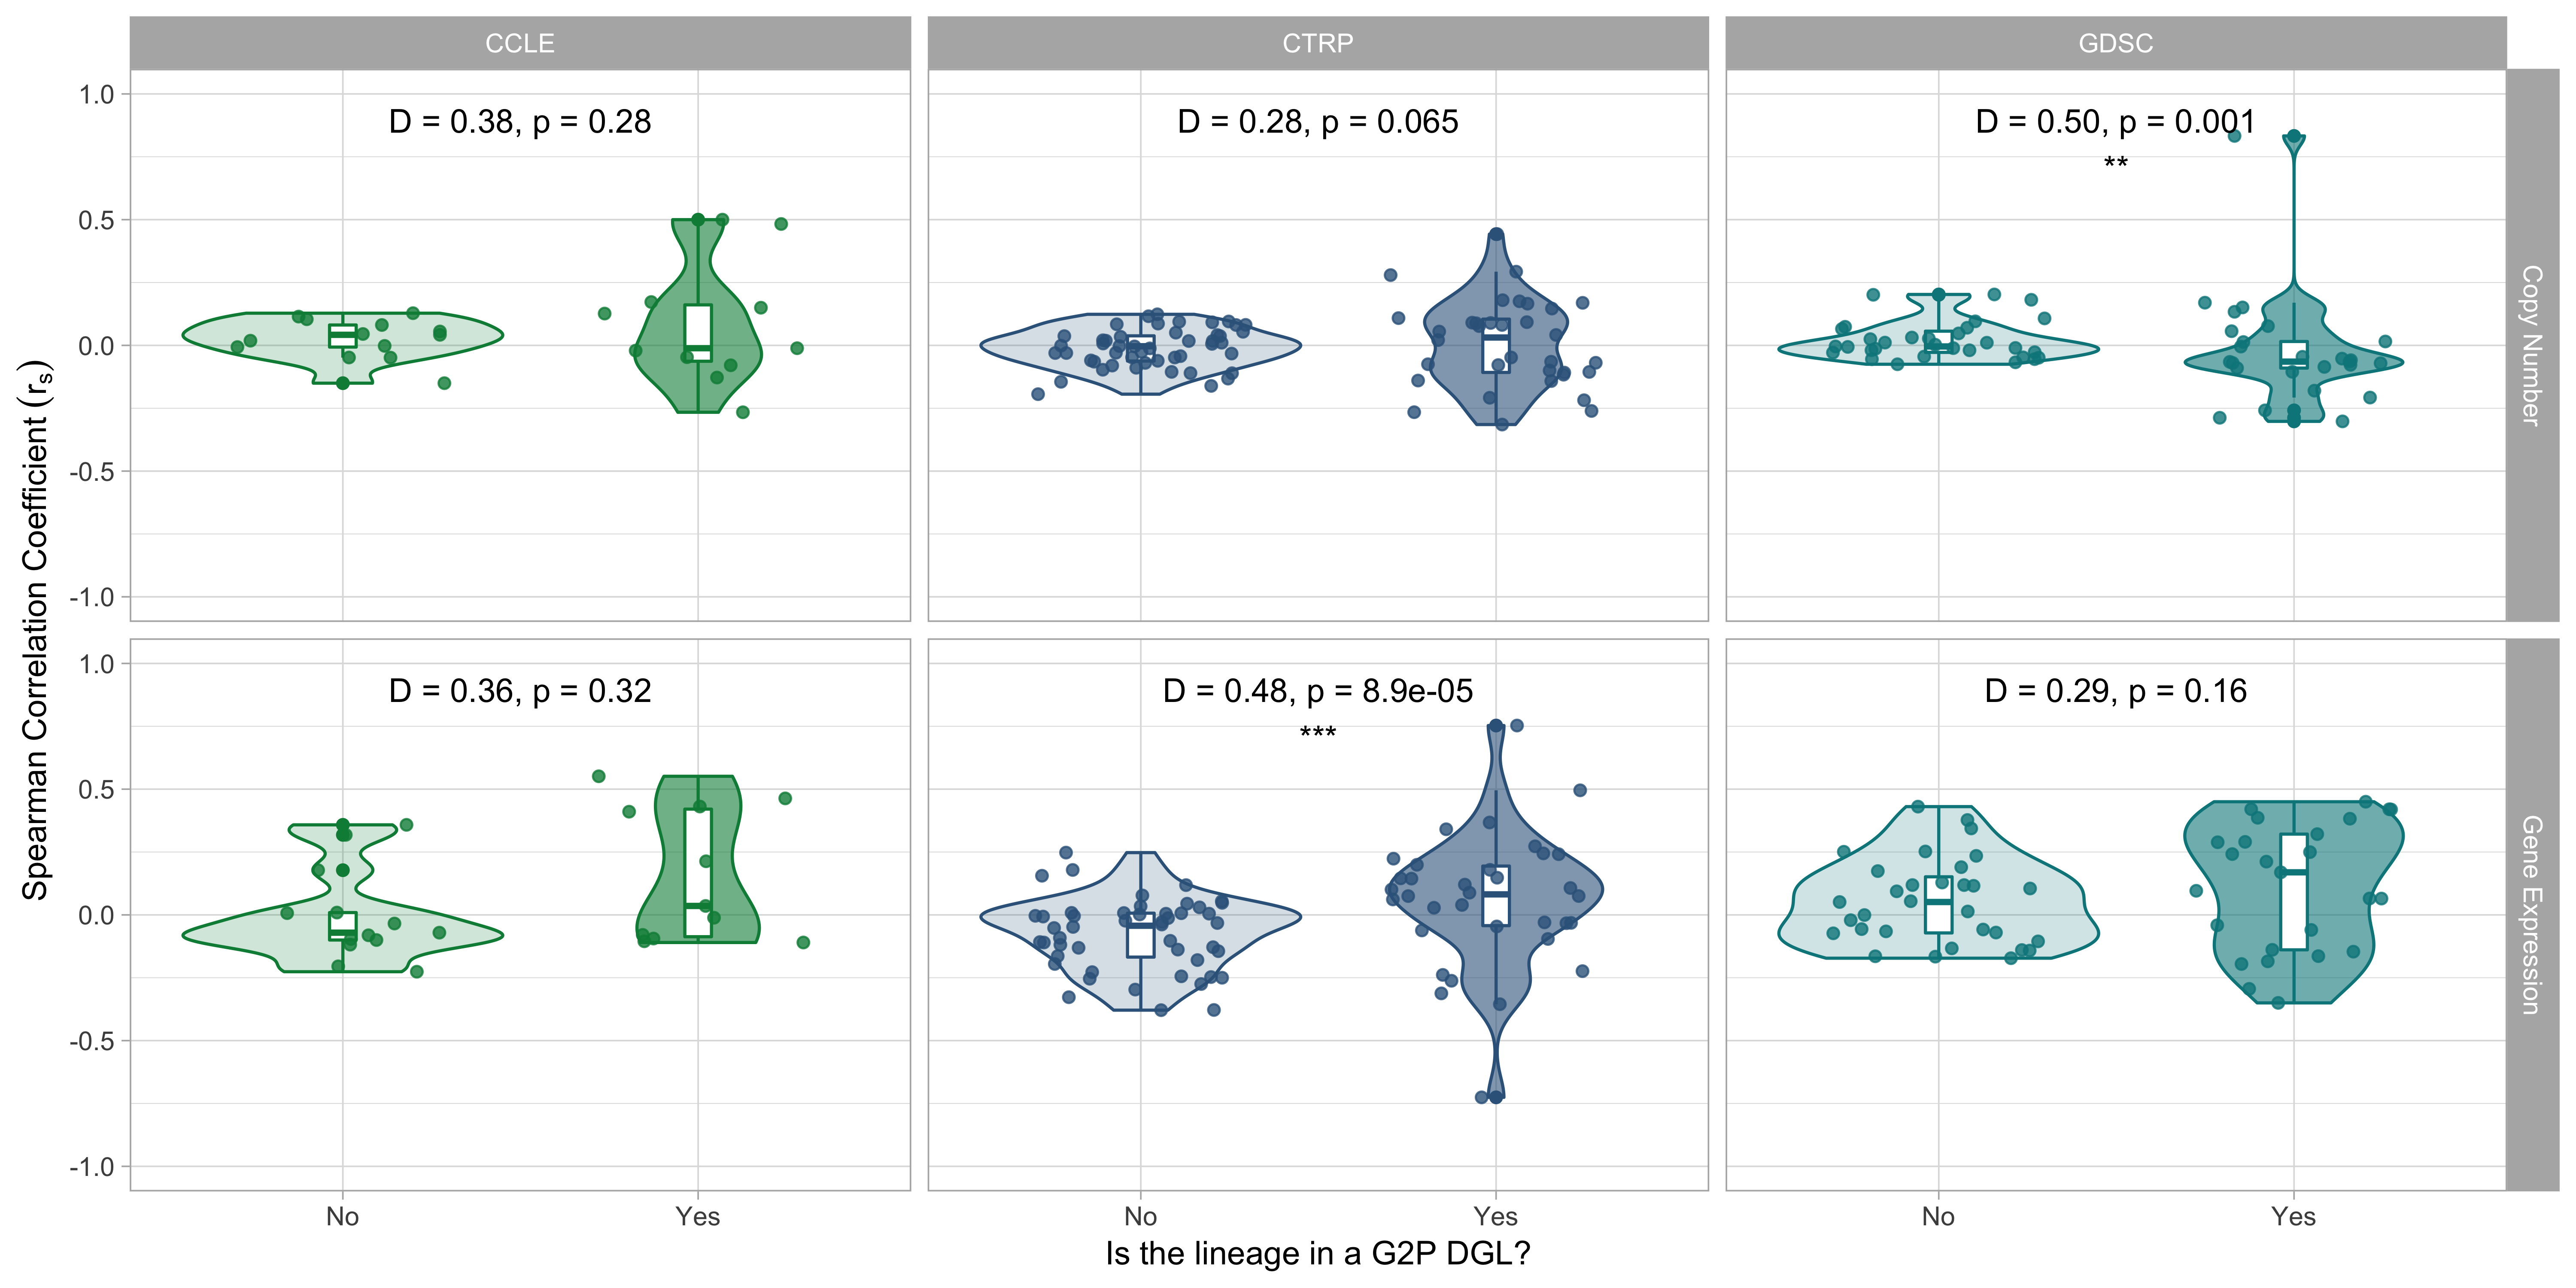
\includegraphics{./plots/manuscript/g2p_spearman_ks_res_plot.png}
\caption{\label{fig:ksplot}Comparison of Spearman correlation coefficients
derived from copy number (log\(_2\) ratio), gene expression (RPKM), and
AUC z-scores from G2P drug-gene associations. Coefficients were grouped
by whether or not the associated lineage for each comparison was in a
G2P drug-gene-lineage association or not. Distributions of these grouped
coefficients were compared using Kolmogorov-Smirnov tests.}
\end{figure}

\subsection{Are CRISPR/Cas9 gene essentiality results comparable to
those of functional drug
screens?}\label{are-crisprcas9-gene-essentiality-results-comparable-to-those-of-functional-drug-screens}

\begin{figure}
\centering
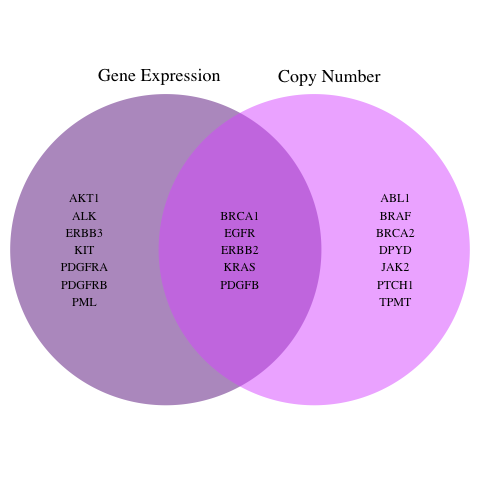
\includegraphics{./plots/manuscript/crispr_venn.png}
\caption{}
\end{figure}

The CRISPR screen from the Broad Institute reports gene dependency using
CERES scores (Meyers et al., 2017), which are generated from sgRNA
depletion scores and eliminate bias arising from the effect of copy
number variation on Cas9 DNA cleavage. The lower the CERES score, the
higher the likelihood that the gene is essential in the associated cell
line. Scores are scaled per cell line such that a score of 0 is the
median effect of nonessential genes and -1 is the median effect of
common core essential genes. Of the 34 G2P genes, only \emph{G6PD} was
not targeted by an sgRNA in the CRISPR dataset.

When we don't account for lineage, Wilcoxon rank-sum tests
(\(p_k = 5.1^{-3}\), FDR \textless{} 5\%) revealed that mutations in 2
genes significantly correlated with CERES score: \emph{KRAS}
(\(p_{adj} = 2.6^{-37}\)) and \emph{BRAF} (\(p_{adj} = 8.2^{-18}\)).
Gene expression (RPKM) of 12 out of 33 (36.36\%) G2P genes significantly
correlated with CERES score, as did copy number (log2-ratio) for 12 out
of 33 (36.36\%) G2P genes (Figure~\ref{fig:crispr-venn}).

For the purpose of comparison to the drug screen data, if we treat
CRISPR knockdown like a small-molecule drug, then these results are more
comprehensive than the results from CCLE, CTRP, and GDSC (Table 2).

\begin{itemize}
\tightlist
\item
  Lineage?
\end{itemize}

\subsection{Are known copy number driven associations recapitulated in
the drug and CRISPR
screens?}\label{are-known-copy-number-driven-associations-recapitulated-in-the-drug-and-crispr-screens}

If a gene's response to is copy number driven, we would expect copy
number to significantly correlate with AUC and gene essentiality scores,
as would gene expression is expression and copy number are associated.

In a lineage-agnostic context of the CRISPR screen, ERBB2 gene
essentiality score had a significant negative correlation with ERBB2
gene expression (\(p < 10^{-12}\), \(r = -0.31\)) and ERBB2 copy number
(\(p < 10^{-15}\), \(r = -0.34\)) (\emph{Figure \#\#2}). Similarly, MET
gene essentiality also correlated with both MET gene expression
(\(p < 10^{-12}\), \(r = -0.31\)) and copy number (\(p < 10^{-8}\),
\(r = -0.25\)). Notably, BRCA1 also significantly correlated with both
gene expression (\(p < 0.001\), \(r = 0.16\)) and copy number
(\(p < 0.01\), \(r = 0.14\)). BRCA2 significantly correlated with all
three of the genomic features tested: gene expression (\(p < 0.05\),
\(r = 0.10\)), copy number (\(p < 10^{-7}\), \(r = 0.23\)), and mutation
status (\(p < 0.001\)).

\subsection{Which genomic features drive KRAS, EGFR, and BRAF drug-gene
associations?}\label{which-genomic-features-drive-kras-egfr-and-braf-drug-gene-associations}

\textbf{Should we do this?}

\section{Discussion}\label{discussion}

Level-A G2P interpretations correspond to clinical evidence that
suggests efficacy of gene targets and/or drugs, and this work questions
whether these relationships manifest themselves in in vitro drug
screens. We have demonstrated that on its own, mutation status is not a
robust predictor of drug efficacy and that copy number and gene
expression fare better as predictors. However, for these three genomic
features in all three datasets, only 11.1\% (mutation status, 1 of 9,
CCLE) to 47.9\% (gene expression, 23 of 48, CTRP) (Table 2), of the
level-A G2P drug-gene associations in the respective dataset were
significant at an uncorrected \(\alpha = 0.05\). This suggests that
while the drug screens successfully identify some clinically relevant
drug-gene associations, many associations are also missed, which raises
the question of the extent to which clinical researchers can rely on in
vitro drug screens when attempting to develop and select therapeutics
for cancer patients.

These results also highlight the need to account for the complex
differences inherent between data generated in clinical scenarios and
data captured in highly controlled, artificial in vitro environments.
Potential sources of variation and error include the fact that cells
growing in a laboratory as opposed to those, even of the same tissue
type, growing in a multicellular organism are exposed to differing sets
of stressors and signals that can significantly impact intracellular
signaling pathways, irrespective of shared genomic profiles. These
differences can include, but are not be limited to, immunologic
reactions, both adaptive and intrinsic (e.g.~cytokine signaling,
inflammation), endocrine (e.g.~stress hormones), and nervous system
stimulation, all of which can have significant downstream implications
on cellular behavior in the context of therapeutic efficacy. Similarly,
a laboratory environment and in vitro cell culture introduce abnormal
growth conditions with respect to extracellular matrix composition,
nutrient availability, and cell density, all of which have the potential
to alter cellular signaling and thus render a drug ineffective during
screening despite would-be in vivo activity.

In the era of precision medicine, the ultimate boon would be that the
unique omics signatures of a patient's individual cancer can be used to
guide treatment. High-throughput, in vitro screens of targeted cancer
agents against cell lines with known omics profiles are beneficial for
testing hypotheses concerning the mechanisms of action for these agents
and they allow for scalability and systematic screening. However,
extrapolating the potential downstream effects of inhibiting a major
growth pathway (e.g.~MAPK, IP-DAG) to predict the clinical prognosis and
progression of a multicellular tumor mass growing in a complex
environment, compounded with the cross-reacting effects of tumor genomic
heterogeneity, make it a questionable statement that one can safely
predict clinical consequences from suppressing a single pathway in a
model system, as evidenced by our findings of fewer than half of the
known clinical associations in the three drug screen datasets. The
benefits of these cancer cell line models, in contrast, lie in their
ability to assess the big-picture effects of these agents. In order to
fully understand therapeutic drug response, a higher degree of
granularity is needed. Additional effort to combine more cell line
information such as gene expression, epigenetic profiles, and proteomic
data with mutational profiles is essential to improving the efficacy and
validity of in vitro cell line screens. Further benefit could be derived
from conducting these screens in environments that are more in line with
the clinical scenarios we are trying to predict. This would include
things such a 3-dimensional cell culture, coculturing with stromal cells
to mimic the tumor microenvironment, as well as other modalities that
can attempt to better replicate in vivo environments.

As a next step to improve the informational granularity of the analysis
presented here, our subsequent goal will be to assess the extent to
which these drug-gene associations are specific to individual cancer
cell line lineages, which are available and annotated in the data sets
analyzed within this report. By evaluating how many clinically
actionable associations are identified in these large-scale functional
screens, we can begin to address best practices for translating
discoveries from these tumor models into clinical trials.

\newpage

\section{Methods}\label{methods}

\subsection{G2P cancer variants}\label{g2p-cancer-variants}

Cancer variants with the highest level of evidence (i.e.~level A) in the
Genotype to Phenotype (G2P) database were retrieved from the Variant
Interpretation for Cancer Consortium (VICC) portal
(\url{https://search.cancervariants.org/\#*}) (A. H. Wagner et al.,
2018) using a customized JSON-query script. All JSON queries were passed
to the available application program interface (API) where a request was
made for all drug-gene associations with level-A evidence via the G2P
evidence label, i.e.~association.evidence\_label. From manual inspection
using G2P's front-end Kibana interface, it was known that, at the time
of the last query, 27 November 2018, there were 1,297 known level-A
associations. Due to the limited request processing capabilities of the
G2P JSON API, queries were batched into packets of 10 data points, for a
total of 130 requests made in succession. Each returned request was
processed as JSON object and searched to identify any existing key:value
pairs for the following variables: evidence level, mutation, gene,
chromosome, start, end, ref, alt, direction, phenotype description,
phenotype family, phenotype ID, drug, drug ID, feature names, and
sequence ID. For any evidence point where a given key:value pair was not
found or unavailable, a value of -1 was assigned. One of the 1,297
level-A entries was irretrievable, yielding a final dataset of 1,296
level-A G2P interpretations, which were stored in a pandas data table
and exported in CSV format. The VICC's methods for the harvesting and
harmonizing of cancer variants is available in a GitHub repository from
Oregon Health \& Science University
(\url{https://github.com/ohsu-comp-bio/g2p-aggregator}).

\subsection{DepMap data retrieval and
processing}\label{depmap-data-retrieval-and-processing}

CRISPR/Cas9, CCLE mutation calls, and CCLE copy number data were all
retrieved from the Broad Institute's Cancer Dependency Map (DepMap)
Public 18Q4 release via the DepMap data portal
(\url{https://depmap.org/portal/download/}) (Broad DepMap, 2018). Gene
expression data was retrieved from the DepMap Public 18Q3 release (Broad
DepMap, 2018) from the same data portal. For cell lines with no CCLE
annotation, the DepMap group drew raw copy number and mutation data from
whole exome sequencing data produced by the Wellcome Trust Sanger
Institute {[}Catalogue Of Somatic Mutations In Cancer (COSMIC,
\url{https://cancer.sanger.ac.uk/cell_lines}) (S. Bamford et al., 2004;
S. A. Forbes et al., 2017); European Genome-phenome Archive (Lappalainen
et al., 2015), accession number EGAD00001001039{]} and processed the
data following the CCLE pipelines to ensure consistency.

\subsubsection{CRISPR/Cas9 screen}\label{crisprcas9-screen}

Gene effect scores for 17,634 genes in 517 cell lines were inferred from
a CRISPR/Cas9 (clustered regularly interspaced short palindromic
repeats/CRISPR-associated 9) screen using the Broad Institute's Avana
knockout library (Doench et al., 2016). The Broad Institute's data
processing and screening methods are available from the figshare record
(Broad DepMap, 2018) and the original publication of CERES, the
algorithm that computes inferred gene dependency scores (Meyers et al.,
2017). The DepMap releases new data quarterly, with the current data set
being the 18Q4 release. This release has 175 more cell lines than the
original data release that was published with CERES (dataset:
gene\_effect.csv, accessed 15 November 2018).

\subsubsection{Mutation calls}\label{mutation-calls}

To preclude variation in genomic feature calls across the datasets, we
used identical annotations from CCLE for all cell lines screened in the
three datasets. The CCLE provided mutation annotations in 19,280 genes
across 1,596 cell lines (dataset: depmap\_18Q4\_mutation\_calls.csv,
accessed 14 November 2018). CCLE called substitutions using MuTect
(Cibulskis et al., 2013) and annotated variants using Oncotator (Ramos
et al., 2015) and indels using Indelocator
(\url{https://software.broadinstitute.org/cancer/cga/indelocator}). We
filtered mutation calls for point mutations, defined as
single-nucleotide insertions, deletions, and substitutions, regardless
of result, i.e.~frameshift, missense, or nonsense mutation. For this
analysis, cell lines harboring non-silent point mutations were
considered \enquote{mutant} for the gene in question. All other
mutations and genes without annotation in the Mutation Annotation Format
(MAF) file were considered \enquote{wildtype.} \enquote{Mutant} and
\enquote{wildtype} calls were binarily encoded per-gene/per-cell line,
regardless of quantity of harbored mutations per gene in a given cell
line.

\subsubsection{Copy number data}\label{copy-number-data}

The CCLE generated genomic copy number (CN) data using the Affymetrix
Genome-Wide Human SNP Array 6.0 and GenePattern pipeline (The Cancer
Genome Atlas Research Network, 2008) and normalized segmented CN
log2-ratios for 23,299 genes across 1,098 cell lines using circular
binary segmentation (Olshen, Venkatraman, Lucito, \& Wigler, 2004)
(dataset: public\_18Q4\_gene\_cn.csv, accessed 15 November 2018).

\subsubsection{Gene expression data}\label{gene-expression-data}

The CCLE reports gene expression in RPKM (reads per kilobase per million
mapped reads) for 54,356 genes across 1,156 cell lines, generated on the
GeneChip Human Genome U133 Plus 2.0 Array (dataset:
CCLE\_DepMap\_18q3\_RNAseq\_RPKM\_20180718.gct, accessed 18 July 2018).

\subsection{Drug screen dataset retrieval and
harmonization}\label{drug-screen-dataset-retrieval-and-harmonization}

The Cancer Therapeutics Response Portal (CTRP) drug screen dataset (v2)
(Basu et al., 2013; M. G. Rees et al., 2016; B. Seashore-Ludlow et al.,
2015) was retrieved from the National Cancer Institute's Cancer Target
Discovery and Development (CTD2) Network's data portal
(\url{https://ocg.cancer.gov/programs/ctd2/data-portal}, accessed 6 June
2018). The Genomics of Drug Sensitivity in Cancer (GDSC) drug screen
dataset (Garnett et al., 2012; Yang et al., 2012) was retrieved from the
data portal at (\url{https://www.cancerrxgene.org/downloads}, accessed
19 June 2018). The Cancer Cell Line Encyclopedia (CCLE) drug screen
dataset (J. Barretina et al., 2012; T. C. C. L. E. Consortium \&
Consortium, 2015) was retrieved from the Broad Institute's data portal
(\url{https://portals.broadinstitute.org/ccle}, accessed 20 June 2018).

\subsubsection{Cell line harmonization}\label{cell-line-harmonization}

In an effort to compare CCLE, CTRP, GDSC and CRISPR results and include
lineage specificity, it was necessary to consolidate cell lines screened
in each dataset. Given that unique identifiers can be used between
studies, it was necessary to standardize the identity of each cell line
with a common source. To achieve this, a freely available cell line
database called Cellosaurus (v26.0, 14 May 2018) (Bairoch, 2018) was
downloaded and merged with the Broad Institute's DepMap cell line data
(accessed 8 June 2018) to create a harmonized cancer cell line database
containing synonymous identifiers that enabled consolidation of all cell
lines used in CCLE, CTRP, GDSC and CRISPR into a common framework.
Subsequent additions to this database include the merging of DepMap IDs
used in the 18Q3 and 18Q4 DepMap data releases. We curated missing
synonyms and identifiers, and we manually annotated the granularity of
lineage labeling for all cell lines analyzed in this study based on
their Human Disease Ontology identity codes (DOIDs,
\url{http://disease-ontology.org/}) (Schriml et al., 2019), resulting in
27 unique lineages. For ease of comparison between datasets, we labeled
all cell lines with custom, randomized identifiers.

\subsubsection{AUC harmonization}\label{auc-harmonization}

The CCLE reports cell line sensitivity to small molecules as an activity
area measured above the dose-response curve (ActArea), while both CTRP
and GDSC report small molecule activity as area under the dose-response
curve (AUC). Since ActArea is reported with a scale of 0 to 8, we
converted CCLE's ActArea values to AUC via

\[AUC=1- \frac{ActArea}{8}\]

All AUC values across the three drug screen datasets were z-score
transformed:

\[z = \frac{AUC - \mu_{AUC}}{\sigma_{AUC}}\]

where AUC is the mean AUC across all drug-cell line combinations in the
dataset and AUC is the standard deviation.

\subsection{Computational}\label{computational}

For \emph{Figure 1}, all data were imported and manipulated using pandas
(v0.23.0) (McKinney, 2011) and plotted using seaborn (v0.90) (Waskom,
2012), which sat on top of matplotlib (v2.2.2) (Hunter, 2007) and was
executed on Python (v2.7.15) (Python Software Foundation,
\url{https://www.python.org/}) in an IPython (v5.5.0) (Pérez \& Granger,
2007) kernel within a localhost Jupyter (v5.2.2) notebook (Kluyver et
al., 2016). All other analyses were conducted in R (v3.5.0) (R
Development Core Team, 2010, \url{https://www.R-project.org/}) in an
RStudio environment (v1.1.447) (RStudio, 2012). All other plots were
drawn using the ggplot2 (v3.0.0) R package (Wickham, 2016).

\subsubsection{Statistics}\label{statistics}

Wilcoxon tests were conducted using the \texttt{compare\_means} function
in the ggpubr (v0.1.7.999) R package (Kassambara, 2018).
\texttt{compare\_means} does Benjamini-Hochberg p-value adjustment using
the \texttt{p.adjust} function from the \texttt{stats} base R package.

For computing Spearman correlation coefficients, we used the
\texttt{cor.test} base R package. If there were 3 or fewer data points,
then the correlation was not done and a value of \texttt{NA} was
supplied.

\newpage

\section{References}\label{references}

\begingroup
\setlength{\parindent}{-0.5in} \setlength{\leftskip}{0.5in}

Finally, the APA guidelines require a note at the start of the reference
section that explains what an asterisk means. This note can be added at
the end of the document as follows.

\hypertarget{refs}{}
\hypertarget{ref-alley1988}{}
Alley, M. C., Scudiere, D. A., Monks, A., Hursey, M. L., Czerwinski, M.
J., Fine, D. L., \ldots{} Boyd, M. R. (1988). Feasibility of Drug
Screening with Panels of Human Tumor Cell Lines Using a Microculture
Tetrazolium Assay. \emph{Cancer Research}, \emph{48}, 589--601.

\hypertarget{ref-bairoch2018}{}
Bairoch, A. (2018). The Cellosaurus, a Cell-Line Knowledge Resource.
\emph{J Biomol Tech}, \emph{29}(2), 25--38.
doi:\href{https://doi.org/10.7171/jbt.18-2902-002}{10.7171/jbt.18-2902-002}

\hypertarget{ref-bamford2004}{}
Bamford, S., Dawson, E., Forbes, S., Clements, J., Pettett, R., Dogan,
A., \ldots{} Wooster, R. (2004). The COSMIC (Catalogue of Somatic
Mutations in Cancer) database and website. \emph{British Journal of
Cancer}, \emph{91}(2), 355--358.
doi:\href{https://doi.org/10.1038/sj.bjc.6601894}{10.1038/sj.bjc.6601894}

\hypertarget{ref-barretina2012}{}
Barretina, J., Caponigro, G., Stransky, N., Venkatesan, K., Margolin, A.
A., Kim, S., \ldots{} Garraway, L. A. (2012). The Cancer Cell Line
Encyclopedia enables predictive modelling of anticancer drug
sensitivity. \emph{Nature}, \emph{483}(7391), 603--607.
doi:\href{https://doi.org/10.1038/nature11003}{10.1038/nature11003}

\hypertarget{ref-basu2013}{}
Basu, A., Bodycombe, N. E., Cheah, J. H., Price, E. V., Liu, K.,
Schaefer, G. I., \ldots{} Schreiber, S. L. (2013). An interactive
resource to identify cancer genetic and lineage dependencies targeted by
small molecules. \emph{Cell}, \emph{154, 154}(5, 5), 1151, 1151--1161.
doi:\href{https://doi.org/10.1016/j.cell.2013.08.003,\%2010.1016/j.cell.2013.08.003}{10.1016/j.cell.2013.08.003, 10.1016/j.cell.2013.08.003}

\hypertarget{ref-ben-david2018}{}
Ben-David, U., Siranosian, B., Ha, G., Tang, H., Oren, Y., Hinohara, K.,
\ldots{} Golub, T. R. (2018). Genetic and transcriptional evolution
alters cancer cell line drug response. \emph{Nature}, \emph{560}(7718),
325--330.
doi:\href{https://doi.org/10.1038/s41586-018-0409-3}{10.1038/s41586-018-0409-3}

\hypertarget{ref-broaddepmap2018a}{}
Broad DepMap. (2018, January 11). DepMap Achilles 18Q4 public. Figshare.
Retrieved from
\url{https://figshare.com/articles/DepMap_Achilles_18Q4_public/7270880}

\hypertarget{ref-broaddepmap2018}{}
Broad DepMap. (2018, January 8). DepMap Achilles 18Q3 public. Figshare.
Retrieved from
\url{https://figshare.com/articles/DepMap_Achilles_18Q3_public/6931364}

\hypertarget{ref-chakravarty2017}{}
Chakravarty, D., Gao, J., Phillips, S., Kundra, R., Zhang, H., Wang, J.,
\ldots{} Schultz, N. (2017). OncoKB: A Precision Oncology Knowledge
Base. \emph{JCO Precision Oncology}, (1), 1--16.
doi:\href{https://doi.org/10.1200/PO.17.00011}{10.1200/PO.17.00011}

\hypertarget{ref-cibulskis2013}{}
Cibulskis, K., Lawrence, M. S., Carter, S. L., Sivachenko, A., Jaffe,
D., Sougnez, C., \ldots{} Getz, G. (2013). Sensitive detection of
somatic point mutations in impure and heterogeneous cancer samples.
\emph{Nature Biotechnology}, \emph{31}(3), 213--219.
doi:\href{https://doi.org/10.1038/nbt.2514}{10.1038/nbt.2514}

\hypertarget{ref-consortium2015}{}
Consortium, T. C. C. L. E., \& Consortium, T. G. of D. S. in C. (2015).
Pharmacogenomic agreement between two cancer cell line data sets.
\emph{Nature}, \emph{528}(7580), 84--87.
doi:\href{https://doi.org/10.1038/nature15736}{10.1038/nature15736}

\hypertarget{ref-doench2016a}{}
Doench, J. G., Fusi, N., Sullender, M., Hegde, M., Vaimberg, E. W.,
Donovan, K. F., \ldots{} Root, D. E. (2016). Optimized sgRNA design to
maximize activity and minimize off-target effects of CRISPR-Cas9.
\emph{Nature Biotechnology}, \emph{34}(2), 184--191.
doi:\href{https://doi.org/10.1038/nbt.3437}{10.1038/nbt.3437}

\hypertarget{ref-domcke2013}{}
Domcke, S., Sinha, R., Levine, D. A., Sander, C., \& Schultz, N. (2013).
Evaluating cell lines as tumour models by comparison of genomic
profiles. \emph{Nat Commun}, \emph{4}.
doi:\href{https://doi.org/10.1038/ncomms3126}{10.1038/ncomms3126}

\hypertarget{ref-forbes2017}{}
Forbes, S. A., Beare, D., Boutselakis, H., Bamford, S., Bindal, N.,
Tate, J., \ldots{} Campbell, P. J. (2017). COSMIC: Somatic cancer
genetics at high-resolution. \emph{Nucleic Acids Res}, \emph{45}(D1),
D777--D783.
doi:\href{https://doi.org/10.1093/nar/gkw1121}{10.1093/nar/gkw1121}

\hypertarget{ref-garnett2012}{}
Garnett, M. J., Edelman, E. J., Heidorn, S. J., Greenman, C. D., Dastur,
A., Lau, K. W., \ldots{} Benes, C. H. (2012). Systematic identification
of genomic markers of drug sensitivity in cancer cells. \emph{Nature},
\emph{483}(7391), 570--575.
doi:\href{https://doi.org/10.1038/nature11005}{10.1038/nature11005}

\hypertarget{ref-geeleher2016}{}
Geeleher, P., Cox, N. J., \& Huang, R. S. (2016). Cancer biomarker
discovery is improved by accounting for variability in general levels of
drug sensitivity in pre-clinical models. \emph{Genome Biology},
\emph{17}, 190.
doi:\href{https://doi.org/10.1186/s13059-016-1050-9}{10.1186/s13059-016-1050-9}

\hypertarget{ref-geeleher2016a}{}
Geeleher, P., Gamazon, E. R., Seoighe, C., Cox, N. J., \& Huang, R. S.
(2016). Consistency in large pharmacogenomic studies. \emph{Nature},
\emph{540}(7631), E1--E2.
doi:\href{https://doi.org/10.1038/nature19838}{10.1038/nature19838}

\hypertarget{ref-greshock2010}{}
Greshock, J., Bachman, K. E., Degenhardt, Y. Y., Jing, J., Wen, Y. H.,
Eastman, S., \ldots{} Wooster, R. (2010). Molecular Target Class Is
Predictive of In vitro Response Profile. \emph{Cancer Research},
\emph{70}(9), 3677--3686.
doi:\href{https://doi.org/10.1158/0008-5472.CAN-09-3788}{10.1158/0008-5472.CAN-09-3788}

\hypertarget{ref-griffith2017}{}
Griffith, M., Spies, N. C., Krysiak, K., McMichael, J. F., Coffman, A.
C., Danos, A. M., \ldots{} Griffith, O. L. (2017). CIViC is a community
knowledgebase for expert crowdsourcing the clinical interpretation of
variants in cancer. \emph{Nature Genetics}, \emph{49}(2), 170--174.
doi:\href{https://doi.org/10.1038/ng.3774}{10.1038/ng.3774}

\hypertarget{ref-haibe-kains2013}{}
Haibe-Kains, B., El-Hachem, N., Birkbak, N. J., Jin, A. C., Beck, A. H.,
Aerts, H. J. W. L., \& Quackenbush, J. (2013). Inconsistency in large
pharmacogenomic studies. \emph{Nature}, \emph{504}(7480), 389--393.
doi:\href{https://doi.org/10.1038/nature12831}{10.1038/nature12831}

\hypertarget{ref-hatzis2014}{}
Hatzis, C., Bedard, P. L., Juul Birkbak, N., Beck, A. H., Aerts, H. J.
W. L., Stern, D. F., \ldots{} Haibe-Kains, B. (2014). Enhancing
Reproducibility in Cancer Drug Screening: How Do We Move Forward?
\emph{Cancer Res}, \emph{74}(15), 4016--4023.
doi:\href{https://doi.org/10.1158/0008-5472.CAN-14-0725}{10.1158/0008-5472.CAN-14-0725}

\hypertarget{ref-haverty2016}{}
Haverty, P. M., Lin, E., Tan, J., Yu, Y., Lam, B., Lianoglou, S.,
\ldots{} Bourgon, R. (2016). Reproducible pharmacogenomic profiling of
cancer cell line panels. \emph{Nature}, \emph{533}(7603), 333--337.
doi:\href{https://doi.org/10.1038/nature17987}{10.1038/nature17987}

\hypertarget{ref-heiser2009}{}
Heiser, L. M., Wang, N. J., Talcott, C. L., Laderoute, K. R., Knapp, M.,
Guan, Y., \ldots{} Spellman, P. T. (2009). Integrated analysis of breast
cancer cell lines reveals unique signaling pathways. \emph{Genome Biol},
\emph{10}(3), R31.
doi:\href{https://doi.org/10.1186/gb-2009-10-3-r31}{10.1186/gb-2009-10-3-r31}

\hypertarget{ref-holbeck2010}{}
Holbeck, S. L., Collins, J. M., \& Doroshow, J. H. (2010). Analysis of
FDA-Approved Anti-Cancer Agents in the NCI60 Panel of Human Tumor Cell
Lines. \emph{Mol Cancer Ther}, \emph{9}(5), 1451--1460.
doi:\href{https://doi.org/10.1158/1535-7163.MCT-10-0106}{10.1158/1535-7163.MCT-10-0106}

\hypertarget{ref-huang2016}{}
Huang, L., Fernandes, H., Zia, H., Tavassoli, P., Rennert, H., Pisapia,
D., \ldots{} Elemento, O. (2016). The cancer precision medicine
knowledge base for structured clinical-grade mutations and
interpretations. \emph{J Am Med Inform Assoc}, \emph{24}(3), 513--519.
doi:\href{https://doi.org/10.1093/jamia/ocw148}{10.1093/jamia/ocw148}

\hypertarget{ref-hunter2007}{}
Hunter, J. (2007). Matplotlib: A 2D graphics environment, \emph{9}(3),
90--95.
doi:\href{https://doi.org/10.5281/zenodo.1202077}{10.5281/zenodo.1202077}

\hypertarget{ref-jang2014}{}
Jang, I. S., Neto, E. C., Guinney, J., Friend, S. H., \& Margolin, A. A.
(2014). Systematic assessment of analytical methods for drug sensitivity
prediction from cancer cell line data. \emph{Pac Symp Biocomput},
63--74. Retrieved from
\url{https://www.ncbi.nlm.nih.gov/pmc/articles/PMC3995541/}

\hypertarget{ref-kassambara2018}{}
Kassambara, A. (2018). Ggpubr: 'Ggplot2' Based Publication Ready Plots
(Version 0.1.7.999). Retrieved from
\url{https://cran.r-project.org/web/packages/ggpubr/index.html}

\hypertarget{ref-kluyver2016}{}
Kluyver, T., Ragan-Kelley, B., Pérez, F., Granger, B., Bussonnier, M.,
Frederic, J., \ldots{} Team, J. D. (2016). Jupyter Notebooks - a
publishing format for reproducible computational workflows. In F.
Loizides \& B. Schmidt (Eds.), \emph{Positioning and Power in Academic
Publishing: Players, Agents and Agendas} (pp. 87--90). IOS Press.

\hypertarget{ref-lappalainen2015}{}
Lappalainen, I., Almeida-King, J., Kumanduri, V., Senf, A., Spalding, J.
D., ur-Rehman, S., \ldots{} Flicek, P. (2015). The European
Genome-phenome Archive of human data consented for biomedical research.
\emph{Nat Genet}, \emph{47}(7), 692--695.
doi:\href{https://doi.org/10.1038/ng.3312}{10.1038/ng.3312}

\hypertarget{ref-marcotte2012}{}
Marcotte, R., Brown, K. R., Suarez, F., Sayad, A., Karamboulas, K.,
Krzyzanowski, P. M., \ldots{} Moffat, J. (2012). Essential gene profiles
in breast, pancreas and ovarian cancer cells. \emph{Cancer Discov},
\emph{2}(2), 172--189.
doi:\href{https://doi.org/10.1158/2159-8290.CD-11-0224}{10.1158/2159-8290.CD-11-0224}

\hypertarget{ref-mcdonald2017}{}
McDonald, E. R., de Weck, A., Schlabach, M. R., Billy, E., Mavrakis, K.
J., Hoffman, G. R., \ldots{} Sellers, W. R. (2017). Project DRIVE: A
Compendium of Cancer Dependencies and Synthetic Lethal Relationships
Uncovered by Large-Scale, Deep RNAi Screening. \emph{Cell},
\emph{170}(3), 577--592.e10.
doi:\href{https://doi.org/10.1016/j.cell.2017.07.005}{10.1016/j.cell.2017.07.005}

\hypertarget{ref-mcfarland2018}{}
McFarland, J. M., Ho, Z. V., Kugener, G., Dempster, J. M., Montgomery,
P. G., Bryan, J. G., \ldots{} Tsherniak, A. (2018). Improved estimation
of cancer dependencies from large-scale RNAi screens using model-based
normalization and data integration.
doi:\href{https://doi.org/10.1101/305656}{10.1101/305656}

\hypertarget{ref-mckinney2011}{}
McKinney, W. (2011). Pandas: A Foundational Python Library for Data
Analysis and Statistics. Retrieved from \url{http://pandas.pydata.org/}

\hypertarget{ref-meyers2017}{}
Meyers, R. M., Bryan, J. G., McFarland, J. M., Weir, B. A., Sizemore, A.
E., Xu, H., \ldots{} Tsherniak, A. (2017). Computational correction of
copy-number effect improves specificity of CRISPR-Cas9 essentiality
screens in cancer cells. \emph{Nat Genet}, \emph{49}(12), 1779--1784.
doi:\href{https://doi.org/10.1038/ng.3984}{10.1038/ng.3984}

\hypertarget{ref-mouradov2014}{}
Mouradov, D., Sloggett, C., Jorissen, R. N., Love, C. G., Li, S.,
Burgess, A. W., \ldots{} Sieber, O. M. (2014). Colorectal Cancer Cell
Lines Are Representative Models of the Main Molecular Subtypes of
Primary Cancer. \emph{Cancer Research}, \emph{74}(12), 3238--3247.
doi:\href{https://doi.org/10.1158/0008-5472.CAN-14-0013}{10.1158/0008-5472.CAN-14-0013}

\hypertarget{ref-neve2006}{}
Neve, R. M., Chin, K., Fridlyand, J., Yeh, J., Baehner, F. L., Fevr, T.,
\ldots{} Gray, J. W. (2006). A collection of breast cancer cell lines
for the study of functionally distinct cancer subtypes. \emph{Cancer
Cell}, \emph{10}(6), 515--527.
doi:\href{https://doi.org/10.1016/j.ccr.2006.10.008}{10.1016/j.ccr.2006.10.008}

\hypertarget{ref-olshen2004}{}
Olshen, A. B., Venkatraman, E. S., Lucito, R., \& Wigler, M. (2004).
Circular binary segmentation for the analysis of array-based DNA copy
number data. \emph{Biostatistics}, \emph{5}(4), 557--572.
doi:\href{https://doi.org/10.1093/biostatistics/kxh008}{10.1093/biostatistics/kxh008}

\hypertarget{ref-patel2017}{}
Patel, S. J., Sanjana, N. E., Kishton, R. J., Eidizadeh, A., Vodnala, S.
K., Cam, M., \ldots{} Restifo, N. P. (2017). Identification of essential
genes for cancer immunotherapy. \emph{Nature}, \emph{548}(7669),
537--542.
doi:\href{https://doi.org/10.1038/nature23477}{10.1038/nature23477}

\hypertarget{ref-patterson2016}{}
Patterson, S. E., Liu, R., Statz, C. M., Durkin, D., Lakshminarayana,
A., \& Mockus, S. M. (2016). The clinical trial landscape in oncology
and connectivity of somatic mutational profiles to targeted therapies.
\emph{Human Genomics}, \emph{10}(1).
doi:\href{https://doi.org/10.1186/s40246-016-0061-7}{10.1186/s40246-016-0061-7}

\hypertarget{ref-paz2003}{}
Paz, M. F., Fraga, M. F., Avila, S., Guo, M., Pollan, M., Herman, J. G.,
\& Esteller, M. (2003). A Systematic Profile of DNA Methylation in Human
Cancer Cell Lines, \emph{63}, 1114--1121.

\hypertarget{ref-perez2007}{}
Pérez, F., \& Granger, B. (2007). IPython: A System for Interactive
Scientific Computing, \emph{9}(3), 21--29.
doi:\href{https://doi.org/10.1109/MCSE.2007.53}{10.1109/MCSE.2007.53}

\hypertarget{ref-rdevelopmentcoreteam2010}{}
R Development Core Team. (2010). \emph{R: A Language and Environment for
Statistical Computing}. Vienna, Austria: R Foundation for Statistical
Computing. Retrieved from \url{https://www.R-project.org/}

\hypertarget{ref-ramos2015a}{}
Ramos, A. H., Lichtenstein, L., Gupta, M., Lawrence, M. S., Pugh, T. J.,
Saksena, G., \ldots{} Getz, G. (2015). Oncotator: Cancer Variant
Annotation Tool. \emph{Human Mutation}, \emph{36}(4), E2423--E2429.
doi:\href{https://doi.org/10.1002/humu.22771}{10.1002/humu.22771}

\hypertarget{ref-rees2016}{}
Rees, M. G., Seashore-Ludlow, B., Cheah, J. H., Adams, D. J., Price, E.
V., Gill, S., \ldots{} Schreiber, S. L. (2016). Correlating chemical
sensitivity and basal gene expression reveals mechanism of action.
\emph{Nat Chem Biol}, \emph{12}(2), 109--116.
doi:\href{https://doi.org/10.1038/nchembio.1986}{10.1038/nchembio.1986}

\hypertarget{ref-rstudio2012}{}
RStudio. (2012). RStudio: Integrated development environment for R
(Version 1.1.447). Boston, MA: RStudio.

\hypertarget{ref-safikhani2016}{}
Safikhani, Z., El-Hachem, N., Smirnov, P., Freeman, M., Goldenberg, A.,
Birkbak, N. J., \ldots{} Haibe-Kains, B. (2016). Safikhani et al. reply.
\emph{Nature}, \emph{540}(7631), E2--E4.
doi:\href{https://doi.org/10.1038/nature19839}{10.1038/nature19839}

\hypertarget{ref-safikhani2017}{}
Safikhani, Z., Smirnov, P., Freeman, M., El-Hachem, N., She, A., Rene,
Q., \ldots{} Haibe-Kains, B. (2017). Revisiting inconsistency in large
pharmacogenomic studies. \emph{F1000Res}, \emph{5}.
doi:\href{https://doi.org/10.12688/f1000research.9611.3}{10.12688/f1000research.9611.3}

\hypertarget{ref-schriml2019}{}
Schriml, L. M., Mitraka, E., Munro, J., Tauber, B., Schor, M., Nickle,
L., \ldots{} Greene, C. (2019). Human Disease Ontology 2018 update:
Classification, content and workflow expansion, 1--8.
doi:\href{https://doi.org/10.1093/nar/gky1032}{10.1093/nar/gky1032}

\hypertarget{ref-seashore-ludlow2015}{}
Seashore-Ludlow, B., Rees, M. G., Cheah, J. H., Cokol, M., Price, E. V.,
Coletti, M. E., \ldots{} Schreiber, S. L. (2015). Harnessing
Connectivity in a Large-Scale Small-Molecule Sensitivity Dataset.
\emph{Cancer Discov}, \emph{5, 5}(11, 11), 1210, 1210--1223.
doi:\href{https://doi.org/10.1158/2159-8290.CD-15-0235,\%2010.1158/2159-8290.CD-15-0235}{10.1158/2159-8290.CD-15-0235, 10.1158/2159-8290.CD-15-0235}

\hypertarget{ref-shoemaker2006}{}
Shoemaker, R. H. (2006). The NCI60 human tumour cell line anticancer
drug screen. \emph{Nature Reviews Cancer}, \emph{6}(10), 813--823.
doi:\href{https://doi.org/10.1038/nrc1951}{10.1038/nrc1951}

\hypertarget{ref-sirota2011}{}
Sirota, M., Dudley, J. T., Kim, J., Chiang, A. P., Morgan, A. A.,
Sweet-Cordero, A., \ldots{} Butte, A. J. (2011). Discovery and
preclinical validation of drug indications using compendia of public
gene expression data. \emph{Sci Transl Med}, \emph{3}(96), 96ra77.
doi:\href{https://doi.org/10.1126/scitranslmed.3001318}{10.1126/scitranslmed.3001318}

\hypertarget{ref-stinson1992}{}
Stinson, S., Alley, M., Kopp, W., Fiebig, H., Mullendore, L., Pittman,
A., \ldots{} Boyd, M. (1992). Morphological and immunocytochemical
characteristics of human tumor cell lines for use in a disease-oriented
anticancer drug screen, \emph{12}(4), 1035--1053.

\hypertarget{ref-tamborero2018}{}
Tamborero, D., Rubio-Perez, C., Deu-Pons, J., Schroeder, M. P.,
Vivancos, A., Rovira, A., \ldots{} Lopez-Bigas, N. (2018). Cancer Genome
Interpreter annotates the biological and clinical relevance of tumor
alterations. \emph{Genome Med}, \emph{10}.
doi:\href{https://doi.org/10.1186/s13073-018-0531-8}{10.1186/s13073-018-0531-8}

\hypertarget{ref-thecancergenomeatlasresearchnetwork2008}{}
The Cancer Genome Atlas Research Network. (2008). Comprehensive genomic
characterization defines human glioblastoma genes and core pathways,
\emph{455}, 1061--1068.
doi:\href{https://doi.org/10.1038/nature07385}{10.1038/nature07385}

\hypertarget{ref-theglobalallianceforgenomicsandhealth2016}{}
The Global Alliance for Genomics and Health. (2016). A federated
ecosystem for sharing genomic, clinical data. \emph{Science},
\emph{352}(6291), 1278--1280.
doi:\href{https://doi.org/10.1126/science.aaf6162}{10.1126/science.aaf6162}

\hypertarget{ref-varley2013}{}
Varley, K. E., Gertz, J., Bowling, K. M., Parker, S. L., Reddy, T. E.,
Pauli-Behn, F., \ldots{} Myers, R. M. (2013). Dynamic DNA methylation
across diverse human cell lines and tissues. \emph{Genome Res},
\emph{23}(3), 555--567.
doi:\href{https://doi.org/10.1101/gr.147942.112}{10.1101/gr.147942.112}

\hypertarget{ref-wagner2018}{}
Wagner, A. H., Walsh, B., Mayfield, G., Tamborero, D., Sonkin, D.,
Krysiak, K., \ldots{} Margolin, A. (2018). A harmonized
meta-knowledgebase of clinical interpretations of cancer genomic
variants. doi:\href{https://doi.org/10.1101/366856}{10.1101/366856}

\hypertarget{ref-wang2015a}{}
Wang, T., Birsoy, K., Hughes, N. W., Krupczak, K. M., Post, Y., Wei, J.
J., \ldots{} Sabatini, D. M. (2015). Identification and characterization
of essential genes in the human genome. \emph{Science},
\emph{350}(6264), 1096--1101.
doi:\href{https://doi.org/10.1126/science.aac7041}{10.1126/science.aac7041}

\hypertarget{ref-waskom2012}{}
Waskom, M. (2012). Seaborn: Statistical data visualization (Version
0.9.0). Retrieved from \url{http://seaborn.pydata.org/}

\hypertarget{ref-weinstein2013}{}
Weinstein, J. N., \& Lorenzi, P. L. (2013). Discrepancies in drug
sensitivity, \emph{504}(7480), 381--313.
doi:\href{https://doi.org/10.1038/504383a}{10.1038/504383a}

\hypertarget{ref-wickham2016}{}
Wickham, H. (2016). Ggplot2: Elegant Graphics for Data Analysis (Version
3.0.0). Retrieved from \url{http://ggplot2.org}

\hypertarget{ref-yang2012}{}
Yang, W., Soares, J., Greninger, P., Edelman, E. J., Lightfoot, H.,
Forbes, S., \ldots{} Garnett, M. J. (2012). Genomics of Drug Sensitivity
in Cancer (GDSC): A resource for therapeutic biomarker discovery in
cancer cells. \emph{Nucleic Acids Res}, \emph{41}(D1), D955--D961.
doi:\href{https://doi.org/10.1093/nar/gks1111}{10.1093/nar/gks1111}

\hypertarget{ref-yu2015}{}
Yu, M., Selvaraj, S. K., Liang-Chu, M. M. Y., Aghajani, S., Busse, M.,
Yuan, J., \ldots{} Neve, R. M. (2015). A resource for cell line
authentication, annotation and quality control. \emph{Nature},
\emph{520}(7547), 307--311.
doi:\href{https://doi.org/10.1038/nature14397}{10.1038/nature14397}

\endgroup


\end{document}
